\subsection{GAN Mel-Spectrogram}
Using the improved Wasserstein GANs framework, we trained generators to
construct 64x64 mel-spectrogram images from a noise vector. Visual results are demonstrated below in Figure~\ref{fig:samples_comparison}.   We saw recognizable Mel-Spectrogram-like features in the
data after only 1000 generator iterations, and after 5000 iterations the generated samples were indistinguishable from real ones. Training took around 10
hours for 20000 iterations on a single 4 GB Nvidia GK104GL GPU.
\begin{figure}[h]
    \centering
    \begin{subfigure}[b]{0.4\textwidth}
        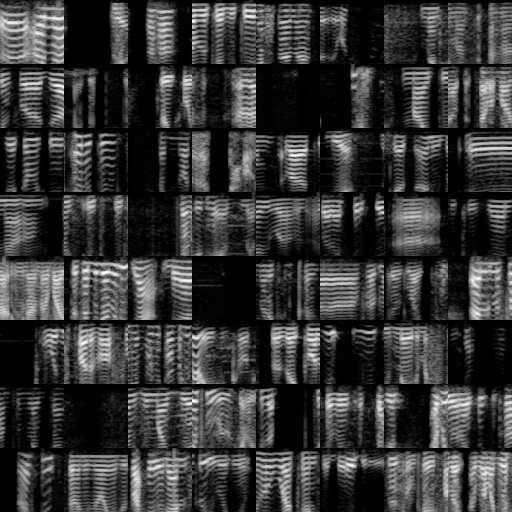
\includegraphics[width=\textwidth]{./fig/samples_groundtruth.png}
        \caption{Real (actual)}
        \label{fig:samples_real}
    \end{subfigure}
    \qquad
    \begin{subfigure}[b]{0.4\textwidth}
        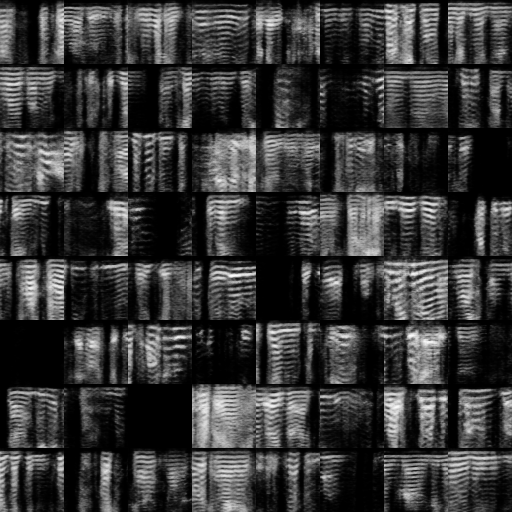
\includegraphics[width=\textwidth]{./fig/samples_5419.png}
        \caption{Fake (generated)}
        \label{fig:samples_fake}
    \end{subfigure}
    \caption{Comparison of real and generated ($\sim$ 5000 generator iterations)
    spectrogram samples from all speakers. Each grid contains 64 samples.}
    \label{fig:samples_comparison}
\end{figure}

\subsection{GAN Adversarial attacks}

Within the GAN framework, we train models for untargeted attacks by using all
data available from speakers that the speaker recognition systems was trained on, 
irrespective of class label. We show that an untargeted model able to generate 
data from the real distribution with enough variety can be used to perform 
adversarial attacks. We provide details in the untargeted attacks 
subsection \ref{sub:untargeted}. Figure~\ref{fig:histogram_untargeted} depicts
that our GAN-trained generator successfully learns all speakers across the
dataset, without mode collapsing.
\begin{figure}[t]
    \centering
    \begin{subfigure}[b]{0.4\textwidth}
        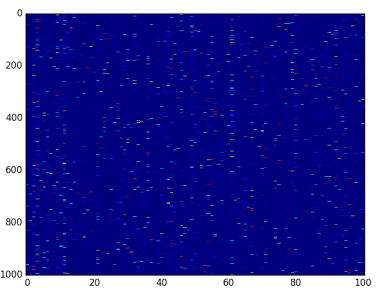
\includegraphics[width=\textwidth]{./fig/conf_mat_untargeted.png}
        \caption{Our speaker classifier's softmax distribution of 1000 samples 
        on approximately 100 speakers.}
        \label{fig:cm_untargeted}
    \end{subfigure}
    \qquad
    \begin{subfigure}[b]{0.4\textwidth}
        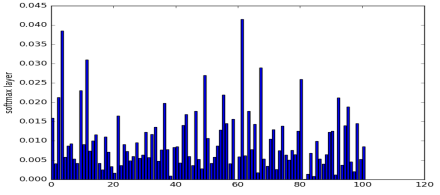
\includegraphics[width=\textwidth]{./fig/histogram_untargeted.png}
        \caption{Our speaker classifier's distribution of randomly sampled 
        speech from the generative model.}
        \label{fig:histogram_untargeted}
    \end{subfigure}
    \qquad
    \begin{subfigure}[b]{0.3\textwidth}
        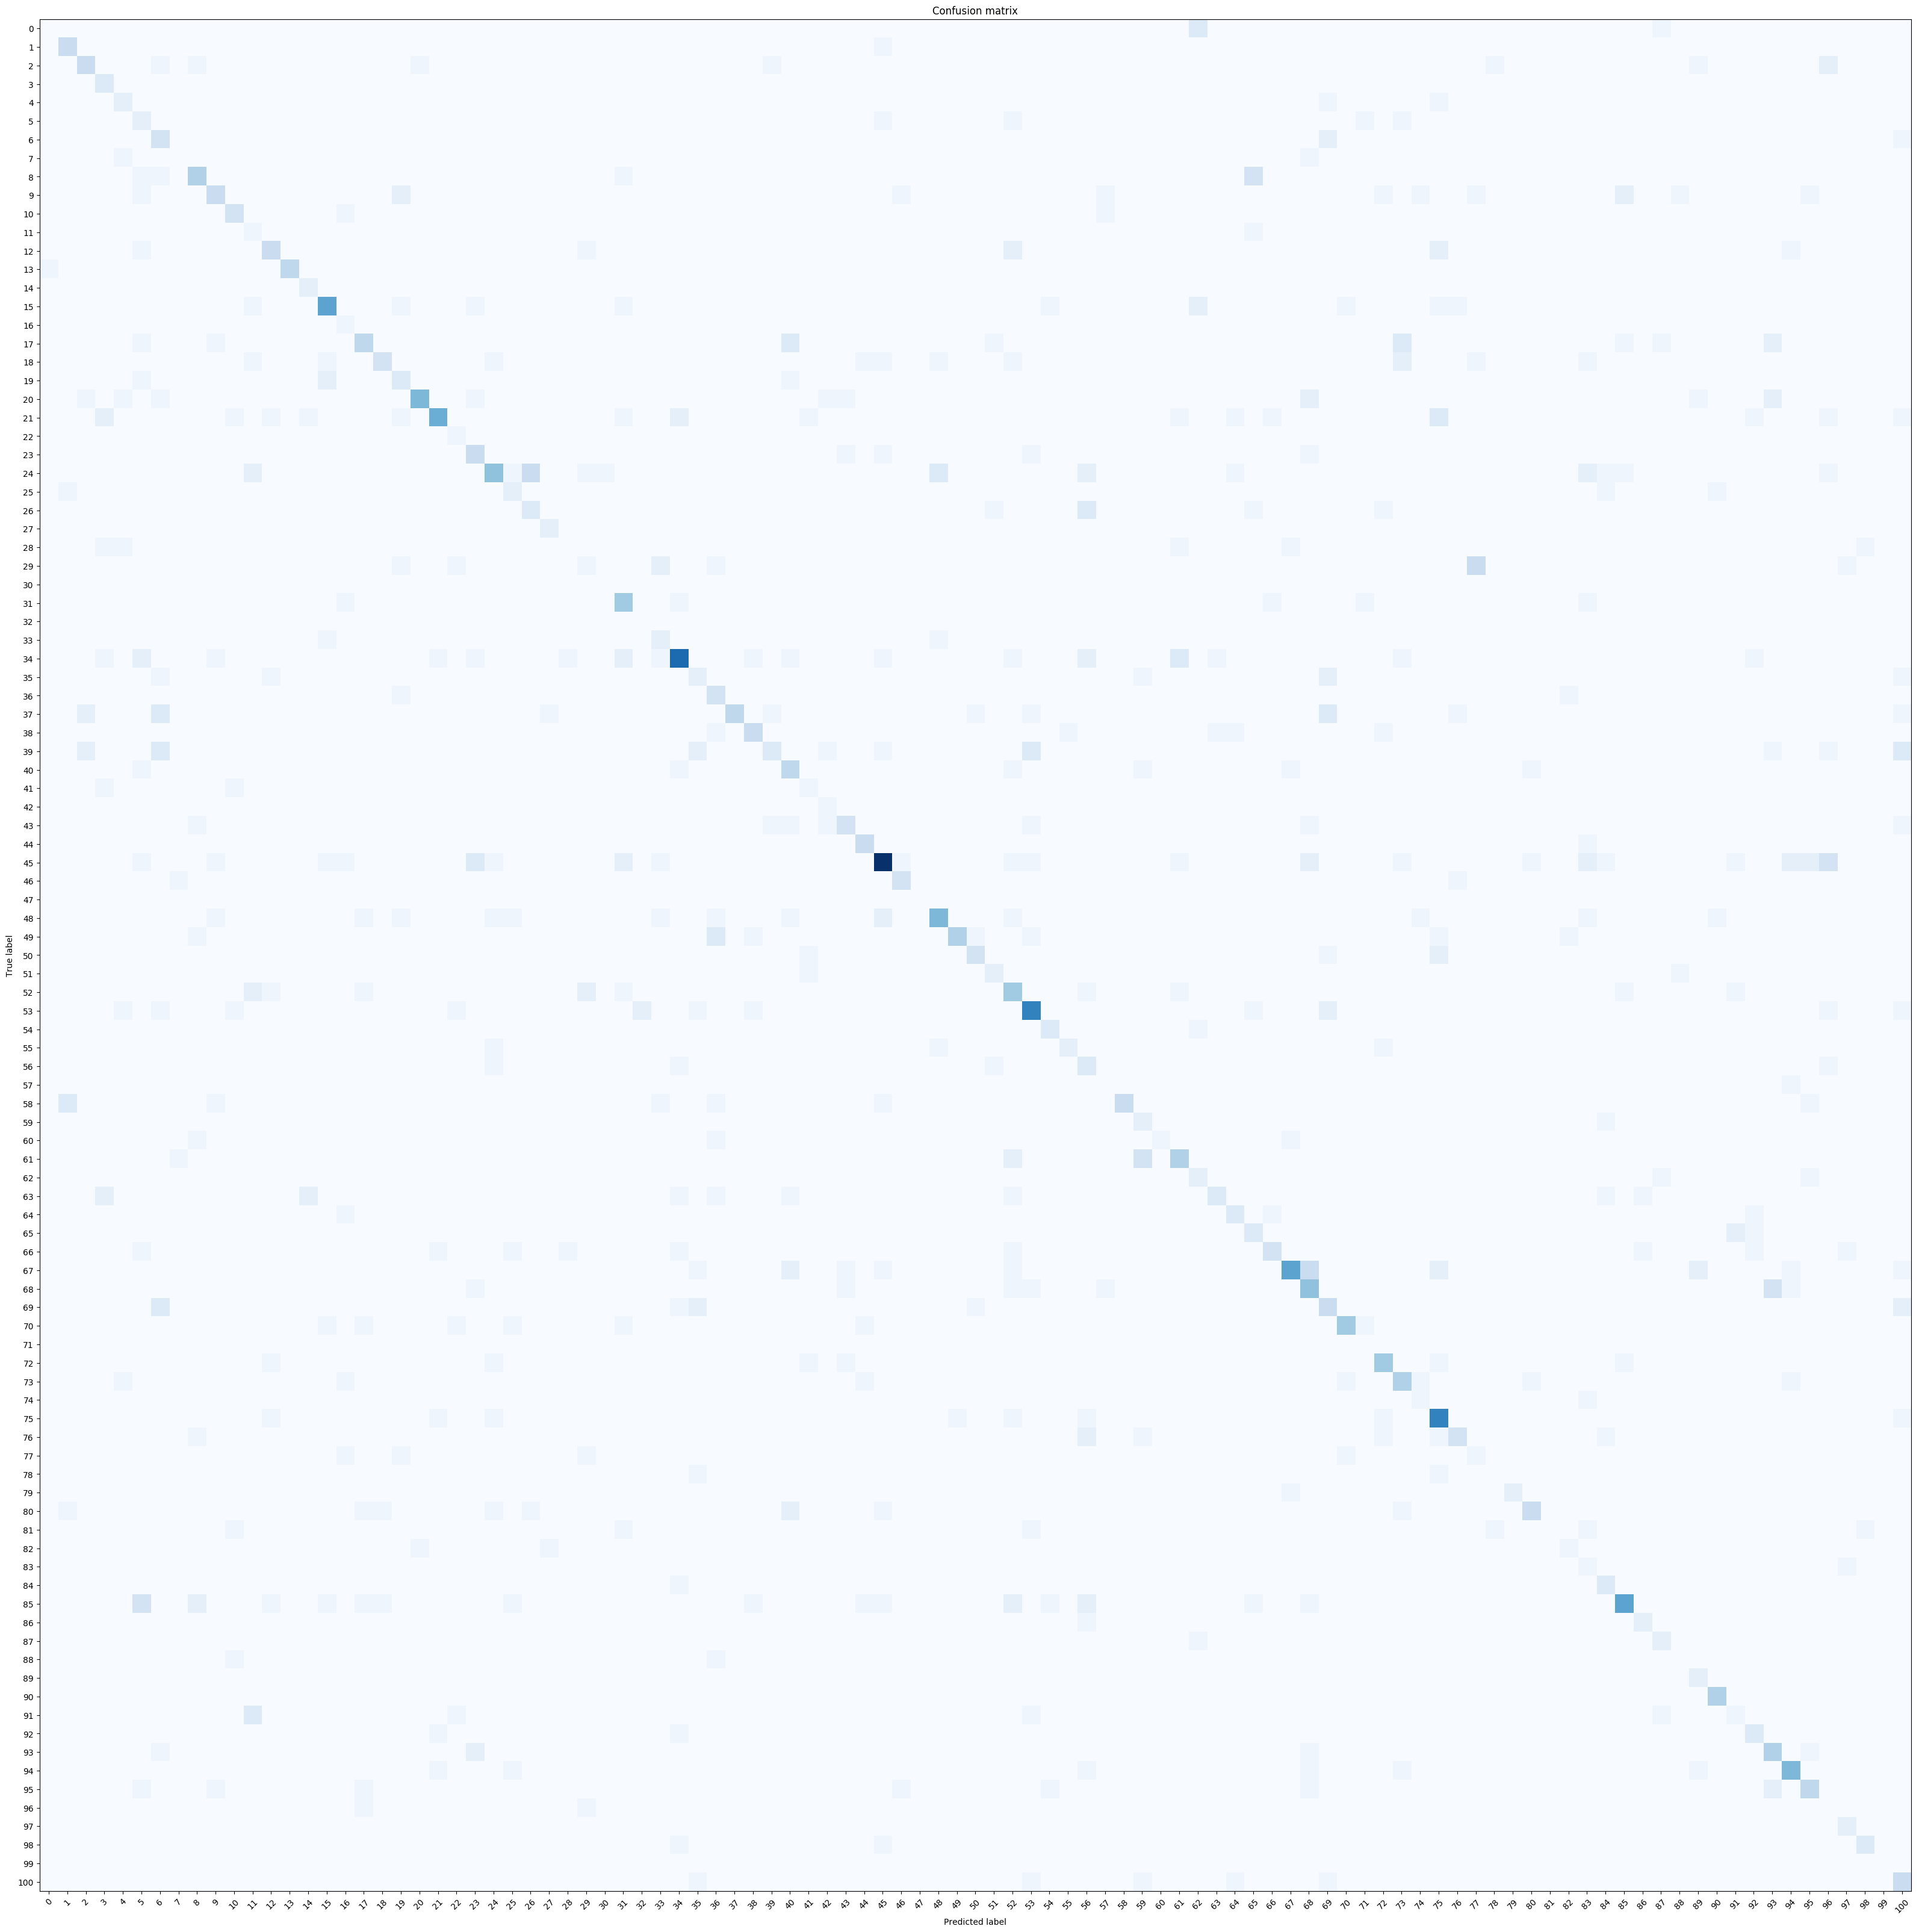
\includegraphics[width=\textwidth]{./fig/conf_mat_cnn_knn.png}
        \caption{Confusion matrix of untargeted model. x-axis corresponds to predicted label, y-axis to ground truth.}
        \label{fig:histogram_untargeted}
    \end{subfigure}
    \caption{Summary of untargeted attacks. Red represents high confidence.}
    \label{fig:conf_mat_cnn_knn}
\end{figure}

As we described earlier, the models for targeted attacks can be trained in two manners: 1) 
conditioning the model on additional information, e.g. class labels, as
described in~\cite{mirza2014conditional}; 2) using only data from the label 
of interest. While the first approach might result in mode collapse, a drawback
of the second approach is that the discriminator, and by consequence the
generator, does not have access to universal\footnote{We draw a parallel with 
Universal Background Models in speech.} properties of speech. In the targeted 
attacks subsection \ref{sub:targeted} we show results using our a new objective function that allows 
using data from all speakers.  

\subsubsection{Untargeted attacks}
\label{sub:untargeted}
For each speaker audio data in the test set, we compute a Mel-Spectrogram as
descibred in section \ref{sub:processdata}. The resulting Mel-Spectrogram is
then fed into the CNN recognizer and we extract a 505-dimensional feature $G$ from
the penultimate fully-connected layer (L7) in the pre-trained CNN model
(\ref{fig:CNN}) trained on the train partition of the real speech dataset with all 
speaker IDs.  This deep feature/embedding $G$ is then used to train a 
K-nearest-neighbor (KNN) classifier, with K equal to 5.

To control the generator trained by our WGAN, we feed the generated
Mel-Spectrograms into the same CNN-L2 pipeline to extract their corresponding
feature $\widehat G$. Utilizing the pre-trained KNN, each sample is assigned to
the nearest speaker in the deep feature space. Therefore, we know which speaker
our generated sample belongs to when we attack our CNN recognizer. We evaluate our
controlled WGAN samples against the state-of-the-art CNN recognizer, and the
confusion matrix can be found in Figure \ref{fig:conf_mat_cnn_knn}. 


\subsubsection{Targeted attacks}
\label{sub:targeted}
We ran all three models (WGAN-GP, SampleRNN, WaveNet) on a mixed corpus containing the entirety of the NIST 2004 corpus, a single speaker (280) from the VCTK Corpus, and the single speaker from the Blizzard dataset. The mixed corpus therefore contains 102 speakers. Samples were created from WaveNet globally conditioned on the single VCTK corpus speaker, and on SampleRNN trained only on data from the Blizzard dataset.
Results are demonstrated in Figure
\ref{fig:confusion_matrices}. Neither WaveNet samples nor sampleRNN samples
were able to attack the recognition model in the same way. In both models, \textbf{none} of the predictions made by the classifier match the target speaker. \\ We also trained the WGAN-GP with mixed loss/without mixed loss on speaker 0. The histogram of predictions in Figure
~\ref{fig:pred_comp_spk0} shows that using the mixed loss model, most of the energy is concentrated on the target speaker 0. The improved WGAN-GP loss achieves 0.38 error
rate and our mixed loss achieves 0.12 error rate, producing a 75\%
increase in accuracy. It is therefore clear that the WGAN-GP mixed loss framework is an improvement on the original loss function, which is expected given the network's access to additional speaker data.

\begin{figure}[t]
    \centering
    \begin{subfigure}[b]{0.3\textwidth}
        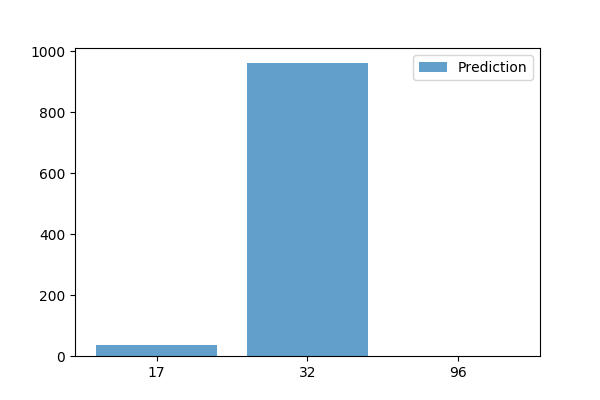
\includegraphics[width=\textwidth]{./fig/pred_histogram_cathy.png}
        \caption{Histogram of sampleRNN predictions. \textbf{Ground truth label: 100}.}
        \label{fig:pred_sampleRNN}
    \end{subfigure}
    \quad
    \begin{subfigure}[b]{0.3\textwidth}
        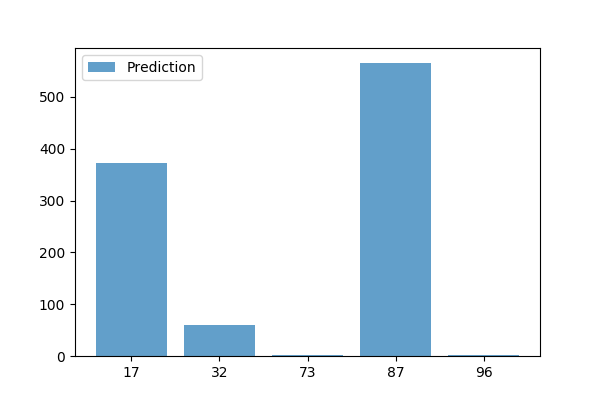
\includegraphics[width=\textwidth]{./fig/pred_histogram_p280.png}
        \caption{Histogram of WaveNet predictions. \textbf{Ground truth label: 101}.}
        \label{fig:pred_wavenet}
    \end{subfigure}
    \quad
    \begin{subfigure}[b]{0.4\textwidth}
        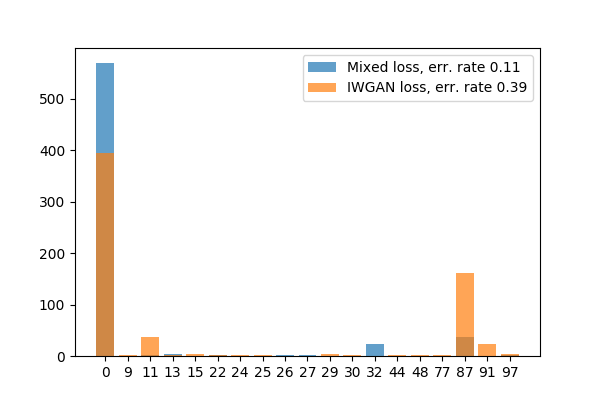
\includegraphics[width=\textwidth]{./fig/pred_comparisson_spk0.png}
        \caption{Histogram of predictions given improved WGAN and mixed loss models.}
        \label{fig:pred_comp_spk0}
    \end{subfigure}
    \caption{Summary histograms of targeted attacks}
    \label{fig:confusion_matrices}
\end{figure}
